\documentclass{article}

\usepackage[utf8]{inputenc}
\usepackage[T1]{fontenc}
\usepackage{hyperref}
\usepackage{url}
\usepackage{booktabs}
\usepackage{amsfonts}
\usepackage{nicefrac}
\usepackage{microtype}
\usepackage[final]{nips_2017}
\usepackage{graphicx}
\usepackage{subcaption}
\usepackage{amsmath}
\usepackage{natbib}
\usepackage{breqn}

\setcitestyle{numbers,open={[},close={]}}
\graphicspath{ {./images/} }

\title{Deep Multimodal Generative Models for Weakly-Supervised Learning}

\author{
    Mike Wu, Noah Goodman \\
    Department of Computer Science \\
    Stanford University \\
    \texttt{{wumike, ngoodman}@cs.stanford.edu} \\
}

\begin{document}

\maketitle

\begin{abstract}
Last thing TODO.
\end{abstract}

\section{Introduction}
The problem of learning from multiple modalities is especially important since the majority of modern information is represented through multiple channels. For example, images in the web are often embedded around text. And while images can be described by pixels, we expect related modalities like text to also hold relevant features. People often interact with this multimodal information in a \textit{bi-directional} way. For example, one can imagine what a black cat looks like but also prescribe this description to a photo. Additionally, available multimodal information is often \textit{sparse}. There exist many large corpuses of images or text alone but few datasets exist (and are expensive to construct) that contain multiple modalities together. Ideally, we would like the generative models we build to extract a joint representation that captures high-level concepts across modalities in a way that is bi-directional and weakly-supervised. 

In this work, we propose a multimodal variational autoencoder (MMVAE), an extension of the traditional VAE framework to handle multiple input types. The first extension is model the setting where we have both an image, $x$, and a natural text, $y$. We then assume a joint generative model of the form $p(x, y, z) = p(z)p(x | z)p(y | z)$ where $p(z)$ is the prior over the latent variable $z$, $p(x | z)$ is our image decoder, and $p(y | z)$ is our text decoder. We then further extend the VAE using a novel objective function, which we call the multimodal ELBO (\textit{MELBO}), for simultaneously training the model from paired data, $D_{p} = \{ (x_{n}, y_{n}) \}$, and unimodal data, $D_{x} = \{ x_{n} \}$, $D_{y} = \{ y_{n} \}$. Namely, using MELBO allows for both evaluating unpaired data at test time and training with sparse paired examples. 

MMVAE jointly fits three encoders: $q(z | x, y)$, $q(z | x)$, and $q(z | y)$. Doing so, we can project images and natural text into the same latent space, and offer ways to translate between the two (bi-directional). For efficiency and simplicity, MMVAEs share parameters between the three encoders. The encoders interact via product of experts (POE) \cite{hinton2006training, vedantam2017generative}. 

We report experimental results on four datasets. The first dataset is MNIST, where labels are stringified to text as the second modality. The second dataset is MultiMNIST, where 0 to 4 MNIST digits are placed on a 50x50 canvas. Unlike the traditional MultiMNIST, we do not vary the locations of these 0 to 4 digits. We again use the stringified label as a the second modality, where the label is the digit class from top-left to bottom-right. The third dataset is the Microsoft COCO Captions dataset \cite{chen2015microsoft}, which contains 330K images and 5 captions per image. The fourth dataset is the LibriSpeech dataset, which contains X waveforms and their text transcriptions. We show that our model performs competitively on these datasets.

Finally, for each of the four datasets, we investigate how our model performs under weak-supervision by aggressively reducing the number of paired data points we provide to the model. We show that MMVAEs do not need a significant number of paired data points to learn a good joint representation across modalities, making this model feasible for real-world tasks i.e. caption generation or speech-to-text. We also briefly discuss reducing the number of data points of a single modality and its effect of learning.

In summary, the contributions of this paper are as follows: first, we present MMVAEs, introducing the MELBO objective. Second, we show that the product of experts techniques works with two unstructured modalities: images and raw text. Lastly, we should that multimodal VAEs are good candidates for weakly supervised learning.

\subsection{Related Work}
In deep learning, multimodal learning is often done using separate branches in the neural net for each modality, and a common top hidden layer. For instance, \citet{ngiam2011multimodal} trained deep autoencoders on audio and video input and found that the bimodal representations were better than any single equivalent. More recently, VAEs \cite{kingma2013auto, kingma2014semi} have been used to train conditional generative models of the form $p(y | x)$ in high-dimensional bimodal settings. Here, $y$ is often a class label, a sentence, or another image depending on the task. For example, conditional VAEs \cite{sohn2015learning}, and conditional multimodal autoencoders (CMMA) \cite{pandey2017variational} maximize a conditional log-likelihood where often one modality is conditioned on another i.e. handwriting digits and labels, faces and attributes, etc. Notably, these CVAEs and CMMAs are not bi-directional. We are more interested in learning a shared latent space of $p(x, y)$ where we can condition interchangeably. 

Recently, there have been several works on such joint models, many of which share commonalities to our proposed model. For example, the BiVCCA employs a similar VAE model with the objective shown below. It includes two inference networks, one for each modality. We note that MMVAE uses a third multimodal objective; we show in our experiments that doing so is important in learning a useful latent space. The BiVCCA loss encourages proper reconstruction of both $x$ and $y$ given only one; $\mu$ acts as a weight to prioritize different modalities. 

\begin{multline}
    J(x, y, \theta, \phi) = \mu (E_{q_{\phi_{x}}(z|x)}[\textup{log}(p_{\theta_{x}}(x|z)) + \lambda \textup{ log}(p_{\theta_{y}}(y|z))] - \textup{KL}(q_{\theta_{x}}(z|x)), p_{\theta}(z)) \\ + (1 - \mu) (E_{q_{\phi_{y}}(z|x)}[\textup{log}(p_{\theta_{x}}(x|z)) + \lambda \textup{ log}(p_{\theta_{y}}(y|z))] - \textup{KL}(q_{\theta_{y}}(z|y)), p_{\theta}(z))
\end{multline}

\citet{suzuki2016joint} then build onto the BiVCCA objective with their JMVAE model, that adds an additional multimodal encoder $q(z|x,y)$ and two additional KL divergence terms to bring $q(z|x,y)$ close to $q(z|x)$ and $q(z|y)$. More explicitly, their objective is the following:

\begin{equation}
    J(x, y, \theta, \phi) = \textup{elbo}_{1, \lambda, 1}(x, y, \theta, \phi) - \alpha[\textup{KL}(q_{\phi}(z|x,y), q_{\phi_{y}}(z|y)) + \textup{KL}(q_{\phi}(z|x,y), q_{\phi_{x}}(z|x))]
\end{equation}

As \citet{vedantam2017generative} note, forcing $q_{\phi(z|y)}$ to be close to $q_{\phi(z|x, y)}$ is somewhat unintuitive but if you rewrite $q_{\phi(z|x, y)}$ as $q_{\phi}^{\textup{avg}}(z|y)$, they show that it has the benefit of $q_{\phi(z|y)}$ covering the embeddings of all $x$ associated with $y$. \citet{vedantam2017generative} go on to introduce their own multimodal VAE objective, the \textit{TELBO} to achieve a similar effect with a simpler design. The TELBO is defined as

\begin{equation}
    J(x, y, \theta_{x}, \theta_{y}, \phi, \phi_{x}, \phi_{y}) = \textup{elbo}_{1, \lambda, 1}(x, y, \theta_{x}, \theta_{y}, \phi) + \textup{elbo}_{1, 1}(x, \theta_{x}, \phi_{x}) + \textup{elbo}_{\gamma, 1}(y, \theta_{y}, \phi_{y})
\end{equation}

where $\lambda, \gamma$ are hyperparameters of the ELBO. See model section for notation. The authors report training this model in two stages: first, using only aligned data, train on first ELBO term alone. Then, freezing the decoders $p_{\theta_{x}}(x|z)$ and $p_{\theta_{y}}(y|z)$, train on the last two ELBO terms above. The TELBO is very similar to our proposed objective (MELBO). We denote three main differences. First, in TELBO, when the input is a single modality, the objective decomposes to the traditional ELBO, where it penalizes differences between the reconstruction and original of that modality only. In MELBO, all three ELBO terms include reconstruction costs for all modalities. For example, given an unpaired image $x$, MELBO encourages its latent representation to decode to both a sensible image and text. We later show that this change is important in produce sharper samples. Second, training MELBO is done concurrently in a single stage. We show paired and unpaired examples together and share encoder and decoder parameters across the three ELBO terms. Thirdly, \citet{vedantam2017generative} only test on images and one-hotted attributes in their experiments. In this work, we will explore a more difficult second modality, unstructured text.  

\section{Methods}
This section first briefly goes over standard VAEs, and product of Gaussians (PoG), then details a new multimodal VAE (MMVAE). See supplement for details of the MLP, CNN, and RNN architectures used as encoders and decoders.

\subsection{Variational Autoencoders}
A variational autoencoder (VAE) \cite{kingma2013auto} is a latent generative model of the form $p_{\theta}(x, z) = p_{\theta}(z)p_{\theta}(x|z)$ where $p_{\theta}(z)$ is usually a Gaussian prior, and $p_{\theta}(x|z)$ is the decoder, representing the likelihood. Training takes the form of fitting an encoder network, $q_{\phi}(z|x)$ to maximize the evidence lower bound (ELBO), defined below:

\begin{equation}\
    \textup{elbo}_{\lambda, \beta}(x, \theta, \phi) = E_{q_{\phi}(z|x, \phi)}[\lambda \textup{ log}(p_{\theta}(x|z))] - \beta \textup{ KL}(q_{\phi}(z|x), p_{\theta}(z))
\end{equation}

$\textup{KL}(p, q)$ is the Kullback Leibler divergence between distributions $p$ and $q$; $\beta$ and $\lambda$ are weights for the different terms in the ELBO. In practice, increasing $\beta$ encourages a better latent embedding but often leads to blurry samples.

\subsection{Product of Experts}

We wish to model the interaction between our modalities as a product of experts \cite{hinton2006training}. Fortunately, because our guide distributions are Gaussian, the product of two Gaussian distributions is itself Gaussian \cite{cao2014generalized}. The resulting Gaussian distribution has mean $\mu = (\sum_{i} \mu_{i}\Sigma^{-1}_{i})(\sum_{i}\Sigma^{-1}_{i})^{-1}$ and covariance $\Sigma = (\sum_{i} \Sigma^{-1}_{i})^{-1}$, where $\mu_{i}$, $\Sigma_{i}$ is the mean and covariance of the $i$-th Gaussian expert. In \cite{hinton2006training}, the prior $p_{\theta}(z)$ is included as an expert for regularization; we omit this term, having found it unstable in practice.

\subsection{Multimodal Variational Autoencoders}

A multimodal variational autoencoder is a model of the form $p_{\theta}(x, y, z) = p_{\theta}(z)p_{\theta}(x|z)p_{\theta}(y|z)$ where $x$ and $y$ are two modalities, i.e. images and text, $z$ is the latent variable, $p_{\theta}(x|z)$ is a image decoder, and $p_{\theta}(y|z)$ is a text decoder. The training objective is as in standard VAE, with the exception that we expand the evidence lower bound definition to include dual modalities.

\begin{multline}
    \textup{elbo}_{\lambda_{x}, \lambda_{y}, \beta}(x, \theta_{x}, \theta_{y}, \phi) = E_{q_{\phi}(z|x, \phi)}[\lambda_{x} \textup{ log}(p_{\theta_{x}}(x|z)) + \lambda_{y} \textup{ log}(p_{\theta_{y}}(y|z))] \\ - \beta \textup{ KL}(q_{\phi}(z|x, y), p_{\theta}(z))
\end{multline}

Note that we have additional hyperparameters, $\lambda_{x}$ and $\lambda_{y}$ that allow us to prioritize one modality over the other. This expanded ELBO is used for paired and unpaired examples. Combining these three terms gives us the Multimodal ELBO (MELBO) objective:

\begin{multline}
    J(x, y, \theta_{x}, \theta_{y}, \phi) = \textup{elbo}_{\lambda_{x}^{1}, \lambda_{y}^{1}, \beta^{1}}(x, y, \theta_{x}, \theta_{y}, \phi) \\ + \textup{elbo}_{\lambda_{x}^{2}, \lambda_{y}^{2}, \beta^{2}}(x, \theta_{x}, \phi) + \textup{elbo}_{\lambda_{x}^{3}, \lambda_{y}^{3}, \beta^{3}}(y, \theta_{y}, \phi)
\end{multline}

The $\lambda$s scale the individual log likelihood terms and the $\beta$s scale the KL divergence terms. We set these parameters using a validation set on a per-dataset level. During training, we shown both paired and unpaired data; and we train the three encoders and decoders together with shared weights. Regardless of paired or unpaired examples, our objective requires both modalities to be reconstructed, sharing parameters for all decoders. We found that this is crucial to learning a good latent space between images and text. This is, to the best of our knowledge, a novel technique. Note that if $\lambda_{y}^{2}$ and $\lambda_{x}^{3}$ are set 0, the MELBO is equivalient to the TELBO \cite{hinton2006training}.

\begin{figure}[h!]
\centering
    \begin{subfigure}[b]{.24\linewidth}
        \centering
        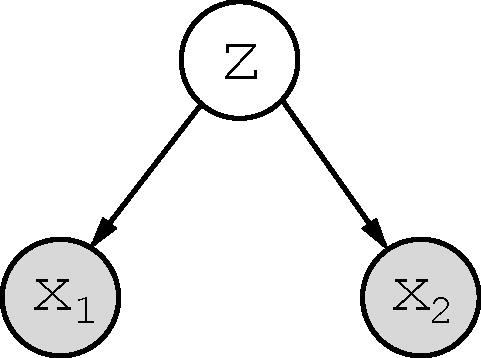
\includegraphics[width=.75\linewidth]{graph.pdf}
        \caption{}
        \label{fig:diagram:graph}
    \end{subfigure}\hspace{5mm}
    \begin{subfigure}[b]{.10\linewidth}
        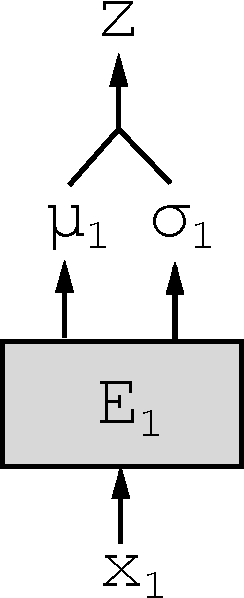
\includegraphics[width=.75\linewidth]{modelv2}
        \caption{}
        \label{fig:diagram:modelv2}
    \end{subfigure}\hspace{5mm}
    \begin{subfigure}[b]{.10\linewidth}
        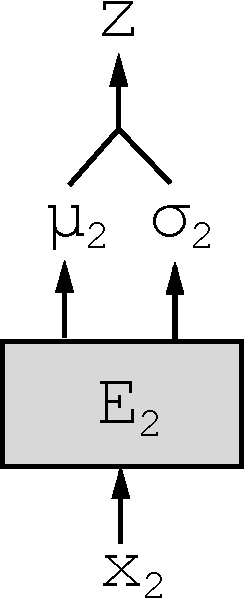
\includegraphics[width=.75\linewidth]{modelv1}
        \caption{}
        \label{fig:diagram:modelv1}
    \end{subfigure}\hspace{5mm}
    \begin{subfigure}[b]{.15\linewidth}
        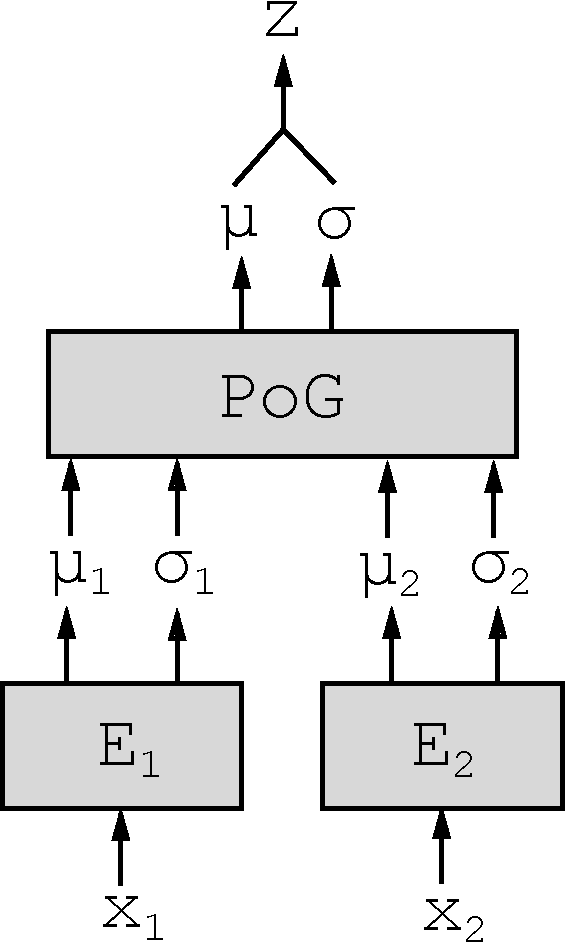
\includegraphics[width=.75\linewidth]{modelv3}
        \caption{}
        \label{fig:diagram:modelv3}
    \end{subfigure}
    \caption{(a) Graphical model of the MMVAE. Gray circles represent observed variables. The white circles represent latent variables. (b) MMVAE when modality 2 is missing. When only 1 modality is present, we ignore the PoG (product of Gaussians). (c) MMVAE when modality 1 is missing. (d) MMVAE when both modalities exist. $E_{1}$ and $E_{2}$ represent the two encoders: $q_{\phi_{x_{1}}}(z | x_{1})$ and $q_{\phi_{x_{2}}}(z | x_{2})$. Regardless if modalities are missing, we optimize the parameters of $E_{1}$ and $E_{2}$.}
    \label{fig:diagram}
\end{figure}

\subsection{Missing Modalities} At training and test time, we can handle missing attributes by using a product of Gaussian experts, as in \cite{hinton2006training}. The inference network takes the form: $q(z|y_{1:k})$. Missing modalities then translates to fewer experts; training proceeds untouched. 

\subsection{Weakly-Supervised Training}
In most circumstances, paired data is both expensive and scarce while unimodal data, i.e. images or text is more easily available in the natural world. The design of MMVAE allows for bootstrapping under sparse labels. During training, we consider input pairs of three types: the first modality alone, the second modality alone, or two paired modalities. Figure \ref{fig:diagram:modelv2}, \ref{fig:diagram:modelv1}, \ref{fig:diagram:modelv3} enumerate these three cases. If given a paired example, use the full MELBO loss. If given only the first modality, decompose the objective to $J(x, \theta_{x}, \phi) = \textup{elbo}_{\lambda_{x}, 0, \beta}(x, \theta_{x}, \phi)$. If given only the second modality, decompose the objective to $J(x, \theta_{y}, \phi) = \textup{elbo}_{0, \lambda_{y}, \beta}(x, \theta_{y}, \phi)$. In other words, when only a single modality is present, use the standard VAE objective. In practice, we find that we only need a limited amount of paired multimodal examples in order to learn the latent space for our datasets.

\section{Experimental Results}

In this section, we fit the MMVAE to four datasets (MNIST, MultiMNIST, COCO-Captions, LibriSpeech) using the MELBO objective. We measure the quality by approximating the marginal log likelihood with a lower bound, and through qualitative analysis of generated samples. We also perform a series of weak-supervision experiments on each dataset, progressively lowering the fraction of paired examples, and unpaired examples and observing performance. 

\subsection{MNIST}

This is the original MNIST dataset except the labels are casted as strings and treated as a separate modality. We use 50k for training, 10k validation, 10k testing. 

\paragraph{Models} We train the MMVAE model using the MELBO objective. We use Adam for optimization with default learning rate of $1e-3$, a minibatch size of 128, 20 latent dimensions, and train for 20 epochs.

For the image encoder, $p(x|z)$ and decoder, $q(z|x)$ we use a three layer MLP with batch normalization and ReLU nonlinearity. For the text encoder $p(y|z)$ and decoder $q(z|y)$, we use a continuous embedding of size 10, and a two layer MLP, again with batch normalization and ReLU. $q(z|y)$ additionally has a softmax to compute probabilities of each word in our vocabulary. The joint decoder, $q(z|x,y)$ is the same as $q(z|y)$, $q(x|y)$ since training shares parameters.

For MELBO parameters, we set $\beta^{i} = 0.004$, and $\lambda_{x}^{i} = \lambda_{y}^{i} = 1, i \in \{1,2,3\}$.

\paragraph{Evaluation} We first measure the marginal log likelihoods, $\textup{log}(p_{\textup{test}}(x))$, $\textup{log}(p_{\textup{test}}(y))$ by computing the ELBO with 1000 particles for importance sampling on 10k test set. For each test example, we can compute the ELBO using both modalities, just images, or just text. This results in 6 marginal probabilities, shown in table. Since MNIST is a prediction task, we can measure the predictive accuracy of our model by generating a text sample conditioned on a image as the label for that image. In table, we measure these nine metrics for a variety of MELBO variations. 

\paragraph{Weak Supervision} We measure the performance of our model on predicting the correct MNIST label as the number of paired examples we show to the model approach 0. We also measure the same performance as the number of unpaired images/text we show approach 0. 

\begin{table}[!h]
    \centering
    \begin{tabular}{ l | c | c }
        Model (MNIST) & $\leq \textup{log }p(x)$ & $\leq \textup{log }p(y)$ \\
        \hline
        VAE & & - \\
        BiVCCA & &  \\
        JMVAE & & \\
        MMVAE (Joint) & & \\
        MMVAE (Image-only) & & \\
        MMVAE (Text-only) & & \\
        MMVAE (Anneal KL) & & \\
        MMVAE (With Universal Expert) & & \\
        MMVAE ($\lambda_{y}^{1} = \lambda_{x}^{1} = 0$) & & \\
        MMVAE ($\lambda_{y}^{2} = \lambda_{x}^{3} = 0$) & & \\
        MMVAE ($\lambda_{x}^{2} = \lambda_{y}^{3} = 0$) & & \\
        MMVAE ($\lambda_{x}^{2} = \lambda_{y}^{2} = \lambda_{x}^{3} = \lambda_{y}^{3} = 0$) & & \\
        \newline
    \end{tabular}
    \caption{TODO}
    \label{table:mnist:marginal}
\end{table}

\begin{figure}[!h]
\centering
    \begin{subfigure}[b]{.24\linewidth}
        \centering
        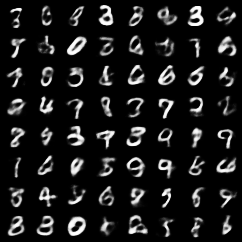
\includegraphics[width=\linewidth]{mnist_mmvae_image_sample.png}
        \caption{}
    \end{subfigure}
    \begin{subfigure}[b]{.24\linewidth}
        \centering
        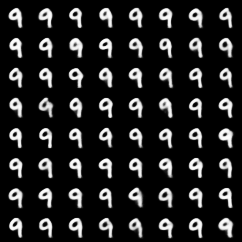
\includegraphics[width=\linewidth]{mnist_mmvae_condition_on_image_text_9_image_sample.png}
        \caption{}
    \end{subfigure}
    \begin{subfigure}[b]{.24\linewidth}
        \centering
        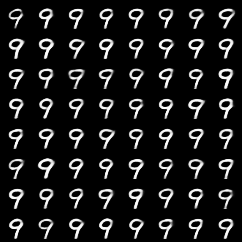
\includegraphics[width=\linewidth]{mnist_mmvae_condition_on_image_9_image_sample.png}
        \caption{}
    \end{subfigure}
    \begin{subfigure}[b]{.24\linewidth}
        \centering
        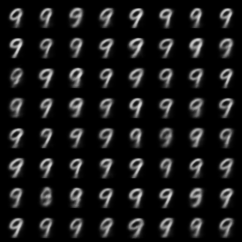
\includegraphics[width=\linewidth]{mnist_mmvae_condition_on_text_9_image_sample.png}
        \caption{}
    \end{subfigure}
    \caption{\emph{MNIST Dataset}: MMVAE is bidirectional, allowing us to try samples unconditionally, or conditioned on modalit(ies) taking a particular value. We note that samples conditioned on both image and text are the most sharp and have the lowest variance. As expected, reconstructed images from text alone are the blurriest. (a) Image samples from $z \sim N(0, 1)$. (b) Image samples from $p(z|x=9,y=9)$. (c) Image samples from $p(z|x=9)$. (d) Image samples from $p(z|y=9)$.}
    \label{fig:mnist:samples}
\end{figure}

\begin{table}[!h]
    \centering
    \begin{tabular}{ l | c | c | c | c | c | c | c | c | c | c | c}
        (a) & 5 & 7 & 1 & 3 & 1 & 6 & 3 & 7 & 5 & 6 & 0 \\
        \hline
        (b) & 9 & 9 & 9 & 9 & 9 & 9 & 9 & 9 & 9 & 9 & 9 \\
        \hline
        (c) & 9 & 9 & 9 & 9 & 9 & 9 & 9 & 9 & 9 & 9 & 9 \\
        \hline
        (d) & 9 & 9 & 9 & 9 & 9 & 9 & 9 & 9 & 9 & 9 & 9 \\
        \newline
    \end{tabular}
    \caption{\emph{MNIST Dataset}: Generated text samples from MMVAE trained on MNIST. (a) Text samples from $z \sim N(0, 1)$. (b) Text samples from $p(z|x=9,y=9)$. (c) Text samples from $p(z|x=9)$. (d) Text samples from $p(z|y=9)$. From (b)-(d), we note that conditioning on an image produces the expected text samples.}
    \label{table:mnist:samples}
\end{table}

\begin{figure}[!h]
\centering
    \begin{subfigure}[b]{.32\linewidth}
        \centering
        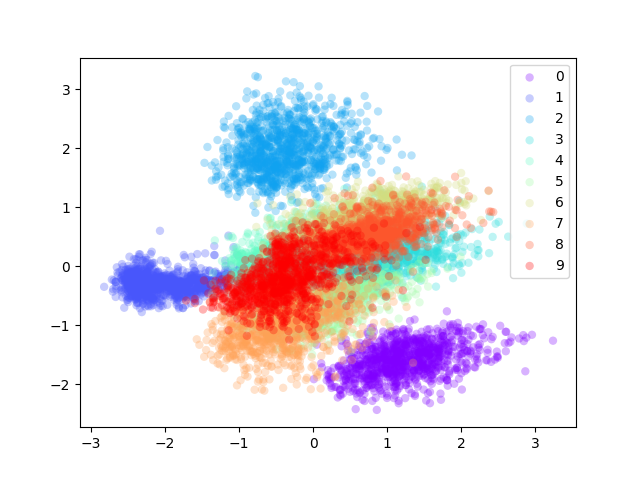
\includegraphics[width=\linewidth]{mnist_mmvae_pca_manifold.png}
        \caption{}
    \end{subfigure}
    \begin{subfigure}[b]{.32\linewidth}
        \centering
        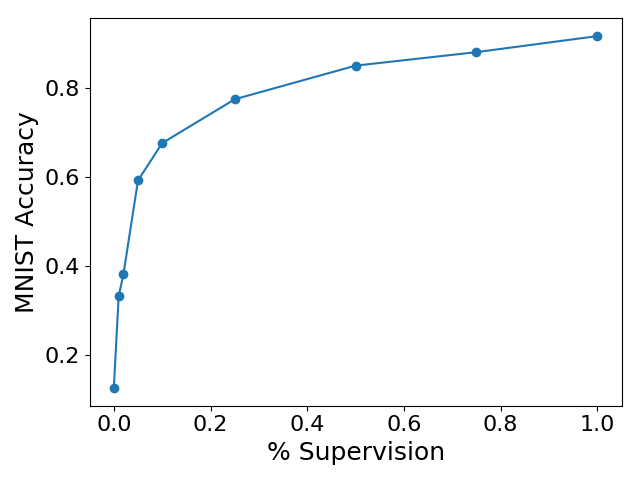
\includegraphics[width=\linewidth]{mnist_mmvae_joint_weak_supervision.png}
        \caption{}
    \end{subfigure}
    \caption{\emph{MNIST Dataset}: (a) Manifold split by MNIST class; this was generated using the top two principal components from 10k latent samples of dimension 20. We can see that each of the classes form a distinct cluster, suggesting that the latent space is well-defined. (b) The effects of weak supervision on the MNIST prediction task where paired data is only shown a fraction of the time; with 25\% supervision, the model reaches 80\% accuracy. TODO: add weak supervision tests for individual modalities.}
    \label{fig:mnist:weaksupervision}
\end{figure}

\subsection{MultiMNIST}

This is a variant of the original MNIST dataset where between 0 and 4 MNIST digits are composed together on a 50x50 canvas. Given a MultiMNIST image, we generate the paired text example by concatenating the digit classes from top-left to bottom-right. Notably, this is a much more difficult text task than our MNIST dataset due to variable text length and a much larger space of acceptable words. We again use 50k for training, 10k for validation, 10k for testing.

\paragraph{Models} Similar training parameters as in MNIST except we use a minibatch size of 64, 100 latent dimensions, and train for 40 epochs due to larger encoder/decoder models.

For the image encoder and decoder, we use the DCGAN architecture from \cite{radford2015unsupervised}. For the text encoder, we use a continuous embedding layer of size 10, followed by a bidirectional GRU with $50$ hidden units, and a single fully connected layer to project into our latent dimension size. For the text decoder, we generate a single character at a time. We include a start token and a stop token in our vocabulary. Generating text is as follows: provided a start token, get its continuous embedding, feed it through a fully connected layer, then a unidirectional GRU, followed by another fully connected layer and a softmax over the 10 character space. We sample a new character and repeat the process until generating a stop token. See supplement for more details.

For MELBO parameters, we anneal $\beta^{i}$ every 5 epochs with the following schedule: 1e-5, 1e-4, 1e-3, 1e-2, 1e-1. We set $\lambda_{y}^{2} = 0.5$ and $\lambda_{x}^{1} = 0.1$. All other $\lambda$s are set to 1.

\paragraph{Evaluation and Weak Supervision} Setup is identical to the MNIST setting except we are measuring (1) that the length of the generated text matches the ground truth, (2) accuracy of matching characters i.e. 2845 and 3845 would be 75\% accuracy, and (3) accuracy of matching sequences i.e. 2845 and 3845 would be incorrect.

\begin{table}[!h]
    \centering
    \begin{tabular}{ l | c | c }
        Model (MultiMNIST) & $\leq \textup{log }p(x)$ & $\leq \textup{log }p(y)$ \\
        \hline
        VAE & & - \\
        BiVCCA & &  \\
        JMVAE & & \\
        MMVAE (Joint) & & \\
        MMVAE (Image-only) & & \\
        MMVAE (Text-only) & & \\
        MMVAE (Anneal KL) & & \\
        MMVAE (With Universal Expert) & & \\
        MMVAE ($\lambda_{y}^{1} = \lambda_{x}^{1} = 0$) & & \\
        MMVAE ($\lambda_{y}^{2} = \lambda_{x}^{3} = 0$) & & \\
        MMVAE ($\lambda_{x}^{2} = \lambda_{y}^{3} = 0$) & & \\
        MMVAE ($\lambda_{x}^{2} = \lambda_{y}^{2} = \lambda_{x}^{3} = \lambda_{y}^{3} = 0$) & & \\
        \newline
    \end{tabular}
    \caption{TODO}
    \label{table:multimnist:marginal}
\end{table}

\begin{figure}[!h]
\centering
    \begin{subfigure}[b]{.24\linewidth}
        \centering
        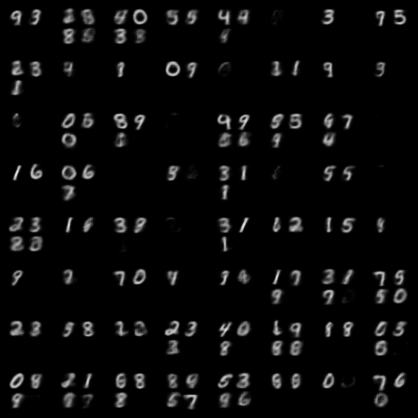
\includegraphics[width=\linewidth]{multimnist_mmvae_image_sample.png}
        \caption{}
    \end{subfigure}
    \begin{subfigure}[b]{.24\linewidth}
        \centering
        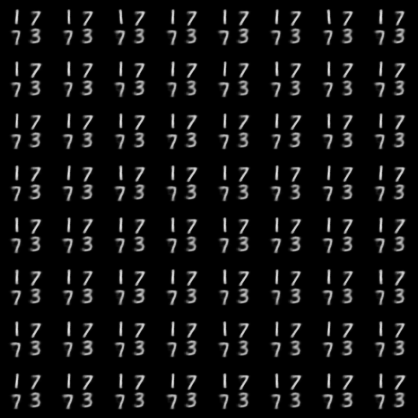
\includegraphics[width=\linewidth]{multimnist_mmvae_condition_image_text_1773_image_sample.png}
        \caption{}
    \end{subfigure}
    \begin{subfigure}[b]{.24\linewidth}
        \centering
        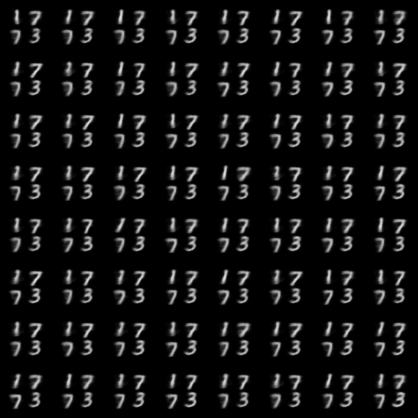
\includegraphics[width=\linewidth]{multimnist_mmvae_condition_text_1773_image_sample.png}
        \caption{}
    \end{subfigure}
    \begin{subfigure}[b]{.24\linewidth}
        \centering
        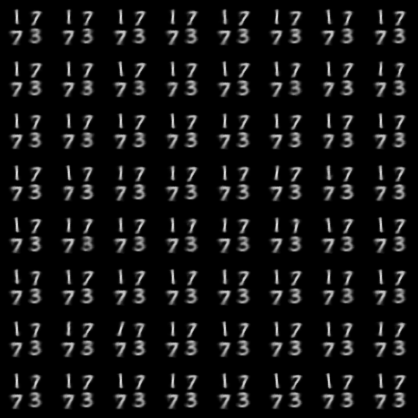
\includegraphics[width=\linewidth]{multimnist_mmvae_condition_on_image_1773_image_sample.png}
        \caption{}
    \end{subfigure}

    \begin{subfigure}[b]{.24\linewidth}
        \centering
        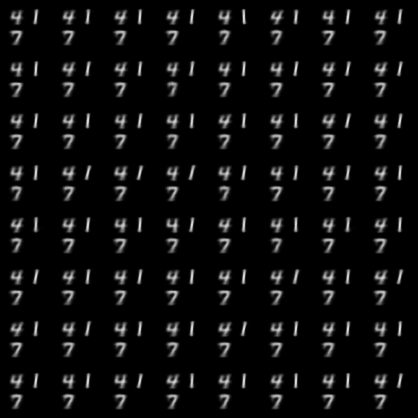
\includegraphics[width=\linewidth]{multimnist_mmvae_condition_on_image_text_417_image_sample.png}
        \caption{}
    \end{subfigure}
    \begin{subfigure}[b]{.24\linewidth}
        \centering
        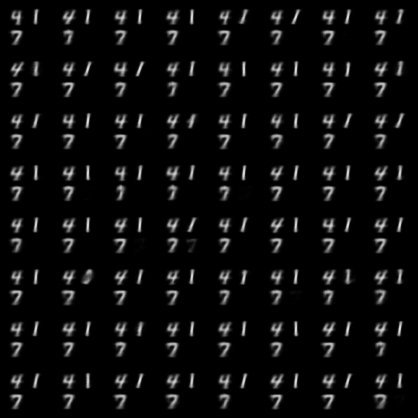
\includegraphics[width=\linewidth]{multimnist_mmvae_condition_on_text_417_image_sample.png}
        \caption{}
    \end{subfigure}
    \begin{subfigure}[b]{.24\linewidth}
        \centering
        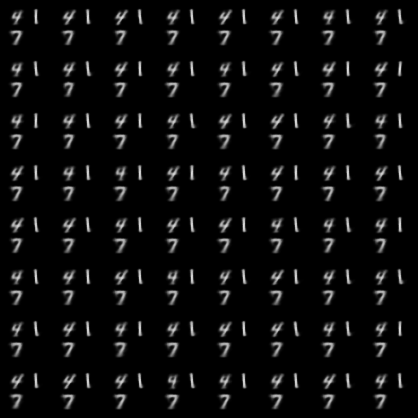
\includegraphics[width=\linewidth]{multimnist_mmvae_condition_on_image_417_image_sample.png}
        \caption{}
    \end{subfigure}

    \begin{subfigure}[b]{.24\linewidth}
        \centering
        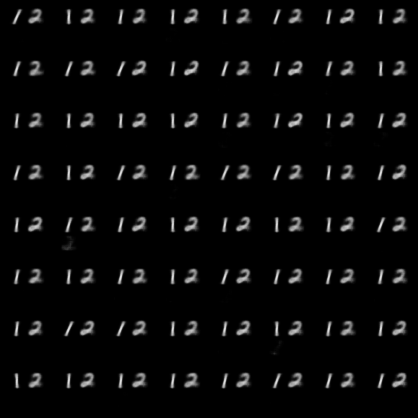
\includegraphics[width=\linewidth]{multimnist_mmvae_condition_on_image_12_image_sample.png}
        \caption{}
    \end{subfigure}
    \begin{subfigure}[b]{.24\linewidth}
        \centering
        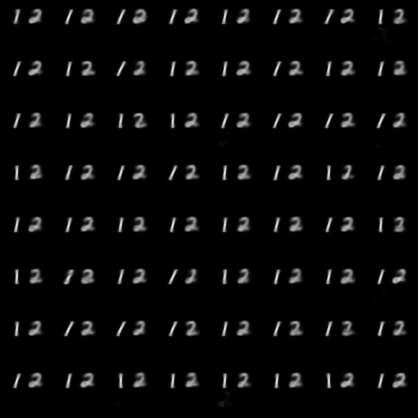
\includegraphics[width=\linewidth]{multimnist_mmvae_condition_on_text_12_image_sample.png}
        \caption{}
    \end{subfigure}
    \begin{subfigure}[b]{.24\linewidth}
        \centering
        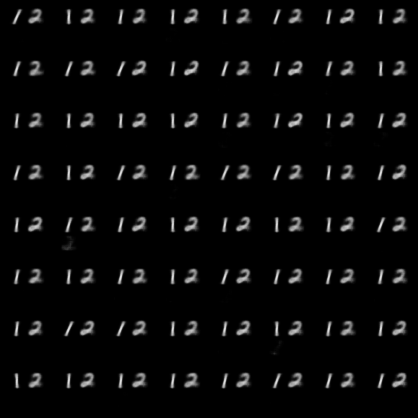
\includegraphics[width=\linewidth]{multimnist_mmvae_condition_on_image_12_image_sample.png}
        \caption{}
    \end{subfigure}

    \caption{\emph{MultiMNIST Dataset}: (a) Image samples from $z \sim N(0, 1)$. (b) Image samples from $p(z|x=1773,y=1773)$. (c) Image samples from $p(z|y=1773)$. (d) Image samples from $p(z|x=1773)$. (e) Image samples from $p(z|x=417,y=417)$. (f) Image samples from $p(z|y=417)$. (g) Image samples from $p(z|x=417)$. (h) Image samples from $p(z|x=12,y=12)$. (i) Image samples from $p(z|y=12)$. (j) Image samples from $p(z|x=12)$. The quality of samples is consistent across number of digits in the canvas. Using image-only, text-only, or both modalities also produce similarly crisp samples.}
    \label{fig:multimnist:samples}
\end{figure}

\begin{table}[!h]
    \centering
    \begin{tabular}{ l | c | c | c | c | c }
        (a) & 93 & 288 & 403 & 9926 & 21 \\
        \hline
        (b) & 1773 & 1773 & 1773 & 1773 & 1773 \\
        \hline
        (c) & 1773 & 1773 & 1773 & 1773 & 1773 \\
        \hline
        (d) & 1773 & 1773 & 1773 & 1673 & 1773 \\
        \hline
        (e) & 417 & 417 & 417 & 417 & 417 \\
        \hline
        (f) & 417 & 417 & 417 & 417 & 417 \\
        \hline
        (g) & 417 & 417 & 417 & 417 & 417 \\
        \hline
        (h) & 21 & 21 & 21 & 21 & 21 \\
        \hline
        (i) & 21 & 21 & 21 & 21 & 21 \\
        \hline
        (j) & 21 & 21 & 21 & 21 & 21 \\
        \newline
    \end{tabular}
    \caption{\emph{MultiMNIST Dataset}: Generated text samples from MMVAE trained on MultiMNIST. (a) Text samples from $z \sim N(0, 1)$. (b) Text samples from $p(z|x=1773,y=1773)$. (c) Text samples from $p(z|x=1773)$. (d) Text samples from $p(z|y=1773)$. (e) Text samples from $p(z|x=417,y=417)$. (f) Text samples from $p(z|y=417)$. (g) Text samples from $p(z|x=417)$. (h) Text samples from $p(z|x=12,y=12)$. (i) Text samples from $p(z|y=12)$. (j) Text samples from $p(z|x=12)$.}
    \label{table:mnist:samples}
\end{table}


\begin{figure}[!h]
\centering
    \begin{subfigure}[b]{.32\linewidth}
        \centering
        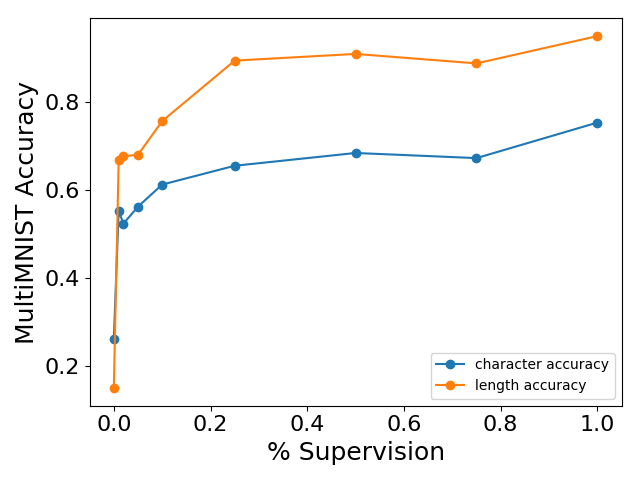
\includegraphics[width=\linewidth]{multimnist_mmvae_joint_weak_supervision.png}
        \caption{}
    \end{subfigure}
    \begin{subfigure}[b]{.32\linewidth}
        \centering
        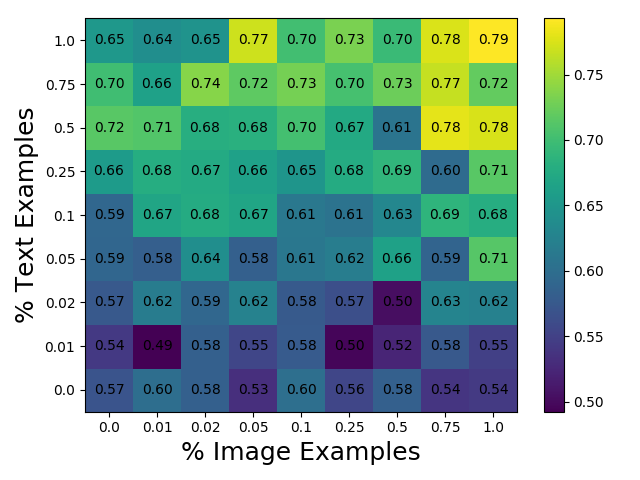
\includegraphics[width=\linewidth]{multimnist_mmvae_modal_char_weak_supervision.png}
        \caption{}
    \end{subfigure}
    \begin{subfigure}[b]{.32\linewidth}
        \centering
        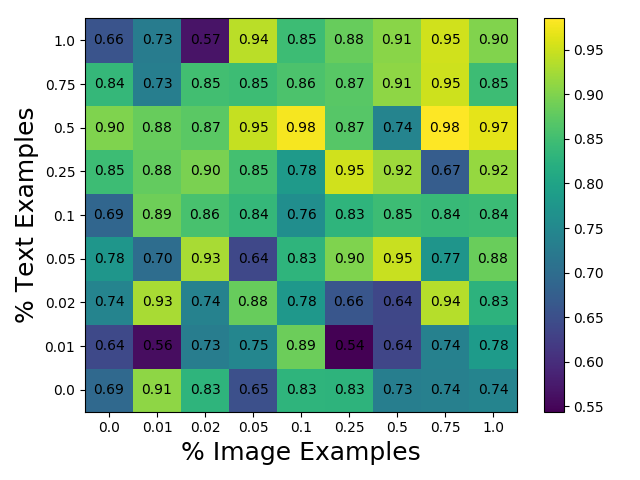
\includegraphics[width=\linewidth]{multimnist_mmvae_modal_length_weak_supervision.png}
        \caption{}
    \end{subfigure}
    \caption{\emph{MultiMNIST Dataset}: a series of weak supervision experiments. (a) Effect of reducing the number of paired examples shown during training. For each image in the test set, generate text conditioned on the image, and measure the number of matching characters (blue line) and the length of text (orange line). The figure shows large gains from 0\% to 10\% supervision with much smaller gains as we approach 100\% supervision, suggesting that MMVAEs do not require a lot of paired data to learn a good latent embedding. (b) Effect of reducing the number of image/text examples on the character prediction task, and (c) on the length prediction task. In (b), the performance is much more sensitive to the number of text samples while in (c), the effect is more balanced between weak image and text supervision. TODO: add embedding pca.}
    \label{fig:multimnist:weaksupervision}
\end{figure}

\subsection{COCO-Captions}

The Microsoft COCO-Captions dataset contains 330k natural images, each tagged with 5 captions. Images are all rescaled to 64x64 and with a 64x64 center crop. When training, every epoch, we randomly sample a caption from the 5 available captions per image. At test time, we use the first caption. We use X for training, X for validation, and X for testing. Both modalities are more difficult than the MultiMNIST setting.

\paragraph{Models} Identical training parameters to MultiMNIST. VAEs suffer from blurry samples when training on natural images. To address this, we replace the DCGAN decoder with a PixelVAE decoder \cite{gulrajani2016pixelvae, oord2016pixel}. For the text encoder and decoders, we increase the hidden units to 500. Instead of learning our own continuous embedding, we use pre-trained GloVe embeddings for each word in our caption to support the large vocabulary size. Generation remains the same with a start and stop token. Identical MELBO parameters to MultiMNIST.

\paragraph{Evaluation and Weak Supervision} There is no predictive task for COCO-Captions. Instead we measure the marginal log likelihood for weak supervision tests. 

\begin{table}[!h]
    \centering
    \begin{tabular}{ l | c | c }
        Model (COCO-Caption) & $\leq \textup{log }p(x)$ & $\leq \textup{log }p(y)$ \\
        \hline
        VAE & & - \\
        BiVCCA & &  \\
        JMVAE & & \\
        MMVAE (Joint) & & \\
        MMVAE (Image-only) & & \\
        MMVAE (Text-only) & & \\
        \newline
    \end{tabular}
    \caption{TODO}
    \label{table:mnist:marginal}
\end{table}

\begin{figure}[!h]
    \centering
    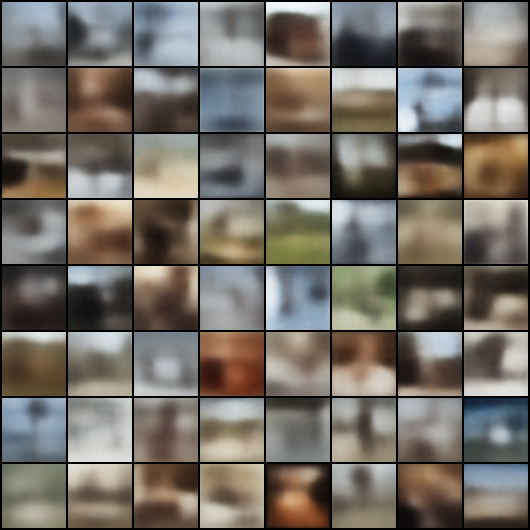
\includegraphics[width=.5\linewidth]{coco_mmvae_image_sample.png}
    \caption{This is a work in progress. These samples were generated with a DCGAN encoder and decoder, hence they are very blurry. However, we can make out coherent structure if we squint. I'm hoping that with a PixelCNN decoder (PixelVAE), we will get sharper samples.}
    \label{fig:WIP:coco:samples}
\end{figure}

\subsection{LibriSpeech}
TODO.

\section{Discussion}
TODO.

\section{Conclusions and Future Work}
TODO.

\bibliographystyle{abbrvnat}
{\small
\linespread{1}
\bibliography{draft}
}

\end{document}